\section{Grade Support and Missing-Grade Structure}
\label{sec:supp_grade_support}

We examine how ordinal transfer changes as target grades receive direct supervision and as the location of missing grades varies. A budget-matched full-support model provides a reference for the adaptation recovered through inheritance.

\subsection{From Missing to Partially Observed Grades}
\label{sec:supp_support_levels}

TIE supplies adaptation to grades without direct training support.

We use three support levels, 0\%, 10\%, and 20\%, under two protocols. The fixed-total protocol keeps the adaptation budget at 256 images while changing the target-grade support. The fixed-seen protocol retains the same seen-grade training images as target-grade support is added. These protocols give complementary views of supervision availability; their exact sample allocations are specified in Sec.~F.3.

Figure~\ref{fig:supp_support_levels} reports the MS-AUC gain of TIE over Adapted. The study covers CoOp-style, OrdinalCLIP-style, and Tip-Adapter-F (CE). Adience and HCI are evaluated under both protocols; FairFace and KonIQ use the fixed-total protocol.

\begin{figure*}[t]
\centering
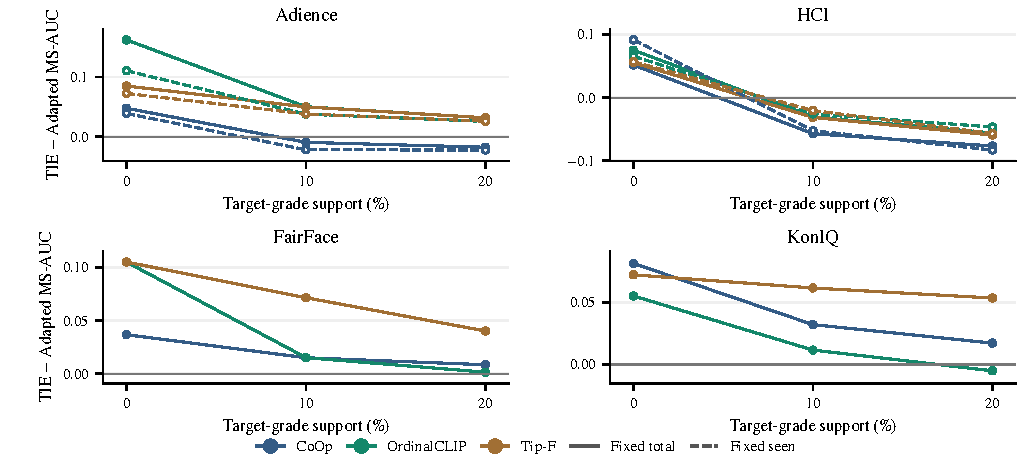
\includegraphics[width=\textwidth]{figures/supp/supp_c_support_levels.pdf}
\caption{\textbf{Sensitivity to grade-specific supervision.}
Change in MS-AUC from Adapted to TIE at 0\%, 10\%, and 20\% target-grade support. Colors distinguish the three adapter configurations. Solid lines use a fixed total training budget; dashed lines retain fixed seen-grade training images. Adience and HCI include both protocols, while FairFace and KonIQ use the fixed-total protocol. Each point is the mean under its corresponding protocol.}
\label{fig:supp_support_levels}
\end{figure*}

All 18 adapter--dataset--protocol trajectories show decreasing average ranking gains from 0\% to 10\% to 20\% support. The largest gains occur when target grades have no images of their own. Once direct supervision is introduced, inheritance contributes less additional information.

On HCI, TIE lowers MS-AUC for all three configurations at 10\% and 20\% target-grade support. Direct supervision reduces the need for inherited displacement, and the benefit of transfer depends on how much a grade has learned from its own images.

\subsection{Endpoints, Interior Grades, and Missing Blocks}
\label{sec:supp_missing_structure}

The main experiments use six missing-grade patterns. Table~\ref{tab:supp_missing_masks} gives their exact grade indices. The notation follows the main paper's one-based grade numbering. Three patterns omit interior grades; the other three involve the label-space endpoints.

\begin{table}[t]
\centering
\caption{\textbf{Missing-grade patterns.}
Grade indices are one-based. HCI and KonIQ share the same $K=5$ masks.}
\label{tab:supp_missing_masks}
\footnotesize
\setlength{\tabcolsep}{3pt}
\begin{tabular*}{\columnwidth}{@{\extracolsep{\fill}}lccc@{}}
\toprule
Pattern & Adience & FairFace & HCI/KonIQ \\
\midrule
Low endpoint & $\{1\}$ & $\{1\}$ & $\{1\}$ \\
Middle & $\{4\}$ & $\{5\}$ & $\{3\}$ \\
High endpoint & $\{8\}$ & $\{9\}$ & $\{5\}$ \\
Adjacent pair & $\{4,5\}$ & $\{4,5\}$ & $\{2,3\}$ \\
Separated pair & $\{2,7\}$ & $\{2,8\}$ & $\{2,4\}$ \\
Both endpoints & $\{1,8\}$ & $\{1,9\}$ & $\{1,5\}$ \\
\bottomrule
\end{tabular*}
\end{table}

\noindent\textbf{Endpoint restoration.}
For a missing endpoint $m$ and its nearest seen grade $n$, TIE copies $D_n$ and exactly recovers the zero-shot margin $T_m-T_n$. This property addresses a measurable adaptation loss. On endpoint patterns, Adapted falls below the zero-shot MS-AUC by 0.065, 0.028, 0.058, and 0.056 on Adience, HCI, FairFace, and KonIQ, respectively. TIE restores the reference ranking for the endpoint--neighbor comparisons.

\noindent\textbf{Interior transfer.}
With seen grades on both sides, inheritance retains information from their adapted displacements. At the original adaptation strength, TIE exceeds zero-shot interior MS-AUC by 0.113 on HCI, 0.025 on FairFace, and 0.096 on KonIQ. Thus, endpoint inheritance restores a reference margin, while interior inheritance can improve upon it.

For consecutive missing grades, equal-weight inheritance gives every grade in the block the same displacement. Their pairwise displacement difference cancels, recovering the zero-shot order within the block. Distance-weighted inheritance instead preserves changes across the anchor interval. Section~\ref{sec:supp_inheritance_rules} analyzes this distinction.

\subsection{Full-Support Reference}
\label{sec:supp_fullsupport}

We compare masked adaptation with FullSup, a budget-matched reference trained with labeled images from every grade. FullSup uses 256 training images and 64 validation images in total, distributed across the complete grade space. The masked models use the same budgets, with training and validation images drawn from seen grades.

FullSup provides a direct-supervision reference for missing-grade performance (Table~2(a) of the main paper). TIE closes 44--58\% of the Missing MAE gap on Adience, HCI, and FairFace. On KonIQ, TIE closes more than the full gap (111\%): its Missing MAE is below FullSup's for eight of nine configurations.

Gap closure is computed within each adapter before averaging, so it can differ slightly from the ratio of the mean errors in main-paper Table~2(a).

Across adapters, the MS-AUC gap-closure ratio has a median of 63\%. One setting is excluded because its FullSup improvement does not meet the reporting criterion in Sec.~\ref{sec:supp_f_metrics}.
